\documentclass{article}
\usepackage[T1]{fontenc}
\usepackage{lmodern}
\usepackage{graphicx}
\usepackage{amsmath,amssymb}
\usepackage[a4paper,margin=2cm]{geometry}
\usepackage[absolute,overlay]{textpos}
\setlength{\TPHorizModule}{1mm}
\setlength{\TPVertModule}{1mm}
\usepackage[indonesian]{babel}
\usepackage{hyperref}
\setlength{\emergencystretch}{2em}
% unit: Halaman 6

\begin{document}

% === Halaman 6 (llm) ===

\begin{itemize}
  \item \textit{One-time pad} (\textit{pad} = kertas bloknot) berisi deretan huruf-huruf kunci yang dibangkitkan secara acak.
\end{itemize}

\vspace{10mm}

Sumber: https://www.cryptomuseum.com/crypto/otp/index.htm

% deskripsi: Foto tangan seseorang yang sedang memegang buku catatan (pad) yang berisi tabel huruf acak untuk metode enkripsi one-time pad.
% bbox normalisasi: [0.2500, 0.2600, 0.7300, 0.8200]
\begin{textblock*}{100.80mm}(52.50mm,77.22mm)
\noindent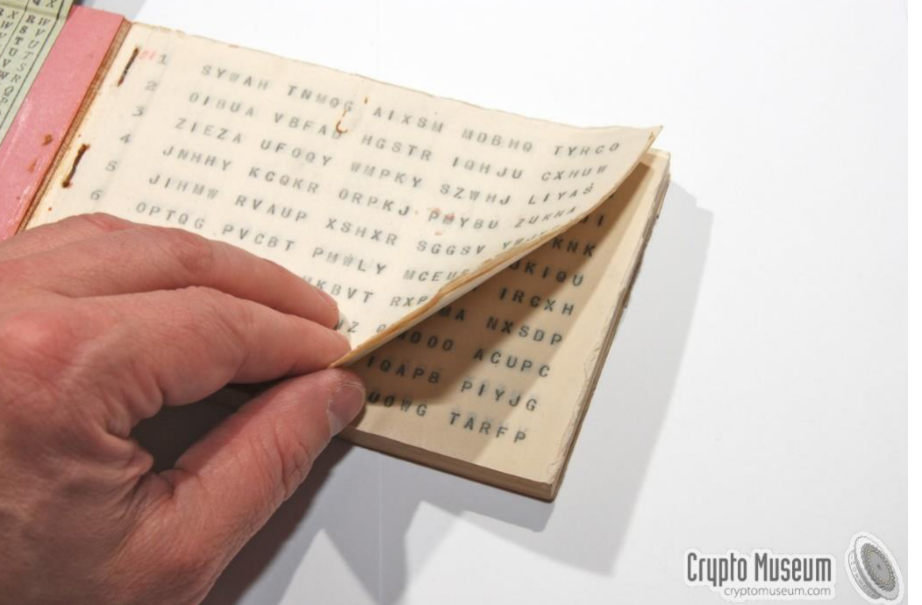
\includegraphics[width=100.80mm,height=166.32mm]{../../images/llm/page_006_img_01.png}%
\end{textblock*}

\end{document}
